\documentclass[11pt,a4paper]{ctexart}
\usepackage[top=1in,bottom=1in,left=1.25in,right=1.25in]{geometry}
\usepackage{graphicx}
\usepackage{tikz}
\usepackage{times,bitmetr}
\usepackage{algorithmic}
\usepackage{algorithm}
\usepackage{array}
\usepackage{mdwmath}
\usepackage{mdwtab}
\usepackage{amsmath}
\usepackage{amsfonts}
\usepackage{amssymb}
%\usepackage{anysize}
\usepackage{subfigure}
\usepackage{pifont}
\usepackage{color}
\usepackage{float}
\usepackage{soul}
\usepackage{tabu}
\bibliographystyle{IEEEtran}



\title{Research Report Four}
\author{Xinpeng Hong
	\thanks{The author acknowledges the support of wavelab in
		making this project a reality}\\
	\\\\
}



% Change to the current month of the series
\reportmonth{October 24}
% Change to the current year of the series
\reportyear{2019}
% Change to the TR number that you obtained from the
% UWEETR web pages when you initially created a new
% TR number. Only provide the last 4 digits here, the year
% goes in the \reportyear{} field above.
\reportnumber{0004}



\begin{document}
\makecover
\maketitle
	

\section{论文阅读}
\subsection{概述}
\noindent 我读了一篇叫Unsupervised Anomaly Detection with Generative Adversarial Networks to Guide Marker Discovery的论文,这是第一篇将GAN思想用于异常检测(图像)的论文。\\
基本思想是:在训练阶段仅利用正常样本在GAN上无监督地学习正常样本的一个在潜在空间中的流形分布,文中为Normal Anatomical Variability,即正常解剖变化,数据为医学图像。在测试阶段读入测试样本,包括正常样本和异常样本,送入GAN中的判别器,寻找一个流形空间内最接近的向量,通过近似程度来决定是否为异常。
\subsection{总结}
\noindent 有个点DCGAN的使用,还有个点是损失函数的选择,之前的论文基本都是直接对辨别器的输出进行损失函数计算,本文为了能获取更丰富的特征信息,作者没有使用这种方法,而是额外利用了辨别器中某一个特征层的输出。\\
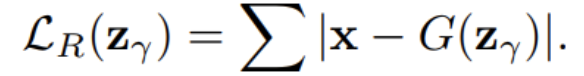
\includegraphics[scale=1]{1.png}\\
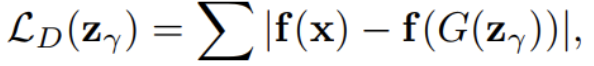
\includegraphics[scale=1]{2.png}\\
\section{代码调试}
\noindent 环境基于python3.7和tensorflow,终端运行程序。\\
\noindent 先通过python download.py mnist把mnist数据集爬下来。\\\\
\noindent 然后训练模型。\\
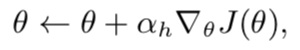
\includegraphics[scale=0.7]{0.png}\\
\noindent 最后测试模型。\\
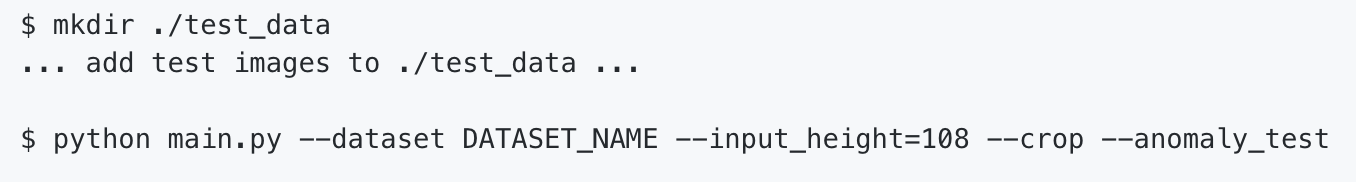
\includegraphics[scale=0.7]{4.png}\\
	
\end{document}